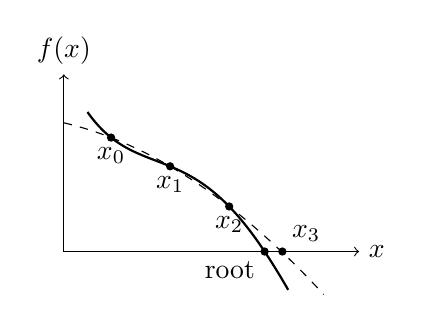
\begin{tikzpicture}[scale=1.5,domain=-.5:1.2]
    \draw[thick] plot[samples=100] (
        \x, {0.3*(\x)^4 - 0.9*(\x)^3 + 0.2*(\x)^2 - 0.4*(\x) + 0.8});
    
    \pgfmathsetmacro{\xzero}{-.3}
    \pgfmathsetmacro{\yzero}{0.3*(\xzero)^4 - 0.9*(\xzero)^3 + 0.2*(\xzero)^2 - 0.4*(\xzero) + 0.8}
    \pgfmathsetmacro{\xone}{0.2}
    \pgfmathsetmacro{\yone}{0.3*(\xone)^4 - 0.9*(\xone)^3 + 0.2*(\xone)^2 - 0.4*(\xone) + 0.8}
    \pgfmathsetmacro{\xtwo}{.7}
    \pgfmathsetmacro{\ytwo}{0.3*(\xtwo)^4 - 0.9*(\xtwo)^3 + 0.2*(\xtwo)^2 - 0.4*(\xtwo) + 0.8}
    \pgfmathsetmacro{\xthree}{1}
    \pgfmathsetmacro{\ythree}{0}
    
    % Draw points
    \fill (\xzero,\yzero) circle (1pt) node[below] {$x_0$};
    \fill (\xone,\yone) circle (1pt) node[below] {$x_1$};
    \fill (\xtwo,\ytwo) circle (1pt) node[below] {$x_2$};
    
    % Compute coefficients for the parabolic interpolation
    \pgfmathsetmacro{\a}{(\yzero/((\xzero-\xone)*(\xzero-\xtwo))) + (\yone/((\xone-\xzero)*(\xone-\xtwo))) + (\ytwo/((\xtwo-\xzero)*(\xtwo-\xone)))}
    \pgfmathsetmacro{\b}{(\yzero*(\xone+\xtwo)/((\xzero-\xone)*(\xzero-\xtwo))) + (\yone*(\xzero+\xtwo)/((\xone-\xzero)*(\xone-\xtwo))) + (\ytwo*(\xzero+\xone)/((\xtwo-\xzero)*(\xtwo-\xone)))}
    \pgfmathsetmacro{\c}{(\yzero*\xone*\xtwo/((\xzero-\xone)*(\xzero-\xtwo))) + (\yone*\xzero*\xtwo/((\xone-\xzero)*(\xone-\xtwo))) + (\ytwo*\xzero*\xone/((\xtwo-\xzero)*(\xtwo-\xone)))}
    
    \draw[dashed] plot[samples=50,domain=-.7:1.5] (
        \x, {\a*(\x)^2 - \b*\x + \c}
    );
    \fill (\xthree,\ythree) circle (1pt) node[below left] {root};
    \fill (1.15,0) circle (1pt) node[above right] {$x_3$};
    % Axes
    \draw[->] (-.7,0) -- (1.8,0) node[right] {$x$};
    \draw[->] (-.7,0) -- (-.7,1.5) node[above] {$f(x)$};
\end{tikzpicture}       
